\chapter{Parte II}

\begin{figure}
\begin{center}
	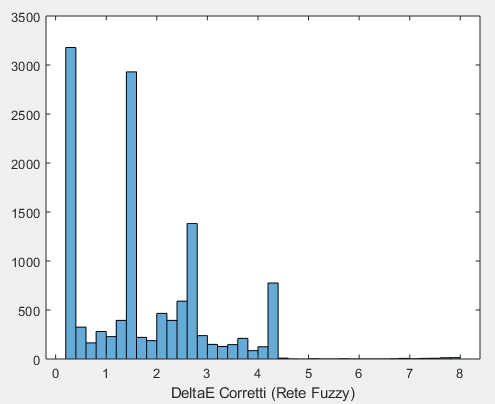
\includegraphics[scale=0.8]{images/rete2-istogramma-deltaecorretti.PNG}
\end{center}
\caption{Istogramma delle DeltaE corrette dalla rete fuzzy)}
\end{figure}

Nella seconda parte delle progetto abbiamo sviluppato una rete neurale che non si limita ad approssimare la formula \ref{eqn:formula} ma tiene conto anche delle diffenze percettive dell'occhio umano. L'equazione infatti è imprecisa per certe zone dello spazio L*a*b e pertanto l'output della rete neurale precedente va corretto. Per fare ciò è necessario passare dallo spazio di colore CIE L*a*b allo spazio di colore CIE L*C*h ed infine definire delle regole di inferenza per un sistema fuzzy di tipo Madamani.
Ricordiamo gli intervalli delle coordinate nello spazio L*C*h.
\begin{itemize}
	\item \textit{Lightness (L)} Range [0, 100]
	\item \textit{Hue (h)} Range  [0, 360\textdegree] 
    \item \textit{Chroma (C)} Il range dipende dal valore L\textsuperscript{*}. \(C\textsubscript{max}= 127\) quando \(L\textsuperscript{*}=50\) cioè quando si è al centro dell'ellellissoide descritto dall spazio L*C*h mentre è \(C\textsuperscript{*}=0\) quando \(L\textsuperscript{*}=0\) oppure \(L\textsuperscript{*}=100\). La relazione tra L\textsuperscript{*} e C\textsubscript{*} quindi si può descrivere come un ellisse.
    	\begin{equation}\label{eqn:ellipse}
       		\frac{C\textsuperscript{*}^2}{127^2} + \frac{(L\textsuperscript{*}-50)^2}{50^2} = 1
       	\end{equation}
\end{itemize}